\section{Results}
\label{sec:results}






\subsection{Comparison of operations}

One means of comparison across the different distance calculation is in how they differ by operation. As discussed in Section~\ref{ssec:ted}, we compare different modification ``operations'', which describe how one tree differs to another. In tree edit distance, this is the sequence of steps taken to modify one tree into another. In the other distance calculations, we can simulate these operations. Unlike tree edit distance, these operations will not necessarily yield a perfectly equivalent tree after modification; however, by counting these ``operations'' per different similarity limit ($\epsilon$) described in Section~\ref{sssec:threshold-problem}, we can better compare how the different distance calculations arrive at their final distance calculation.

We can see this comparison in Figure~\ref{fig:operations}, the distribution of operations for the exp[er]

\begin{figure}
\begin{tabular}{lccc}
    Distance & AT1                                                                         & AT1 vs AT2                                                                    & AT2                                                                         \\
    LD       & 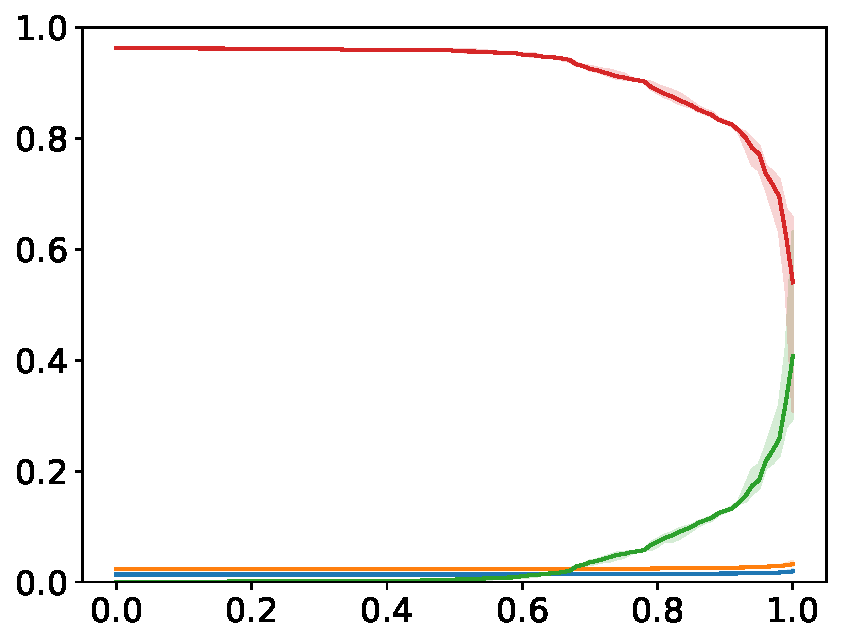
\includegraphics[width=.25\linewidth]{code/img/operation_count_ld_AT1.pdf}  & 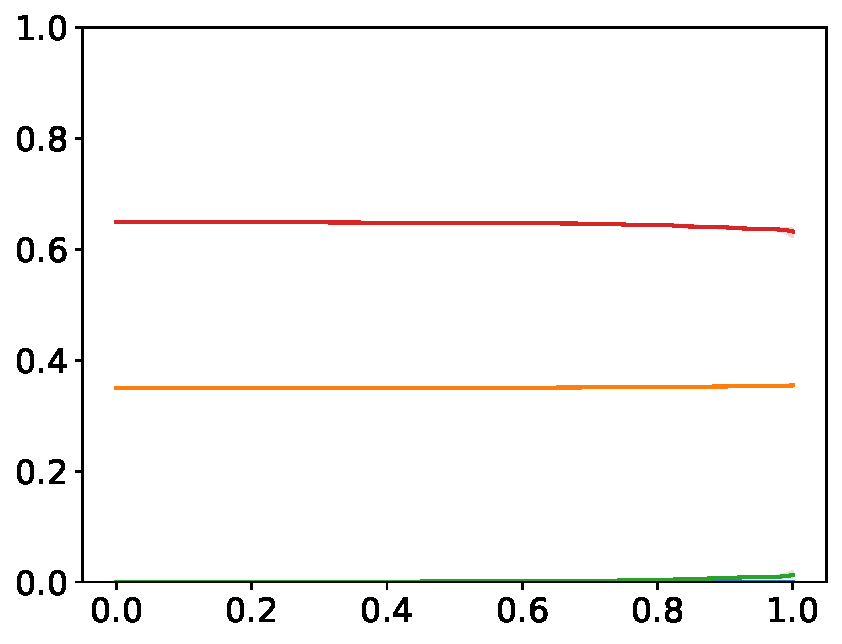
\includegraphics[width=.25\linewidth]{code/img/operation_count_ld_AT1-2.pdf}  & 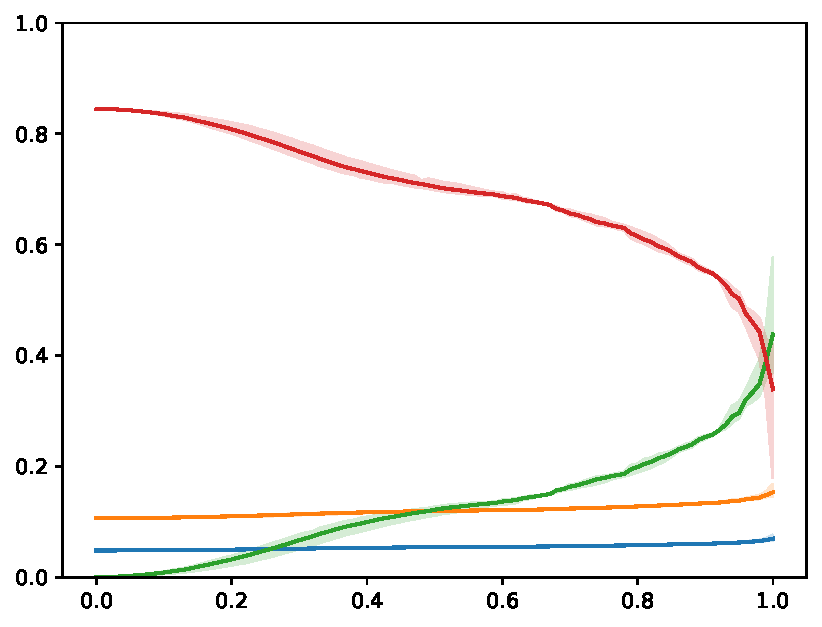
\includegraphics[width=.25\linewidth]{code/img/operation_count_ld_AT2.pdf}  \\
    TED      & 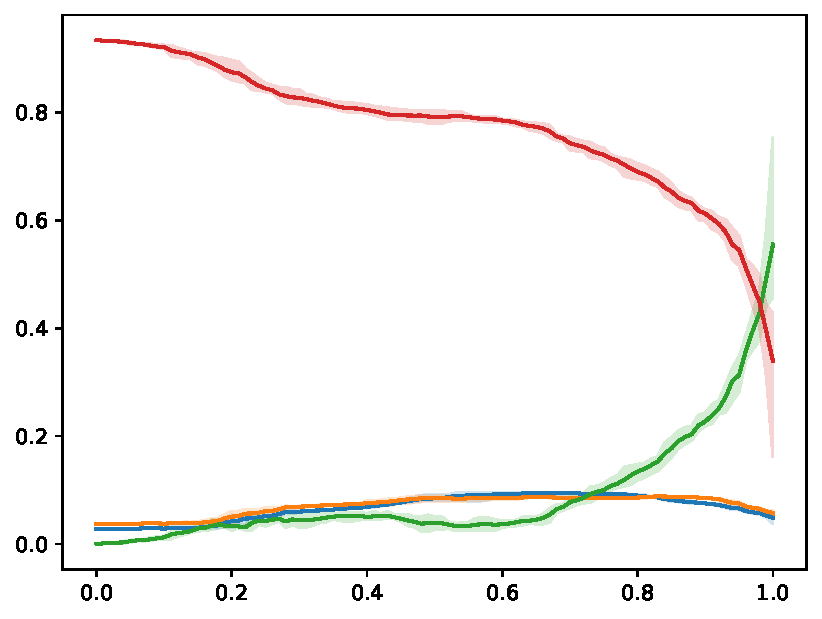
\includegraphics[width=.25\linewidth]{code/img/operation_count_zss_AT1.pdf} & 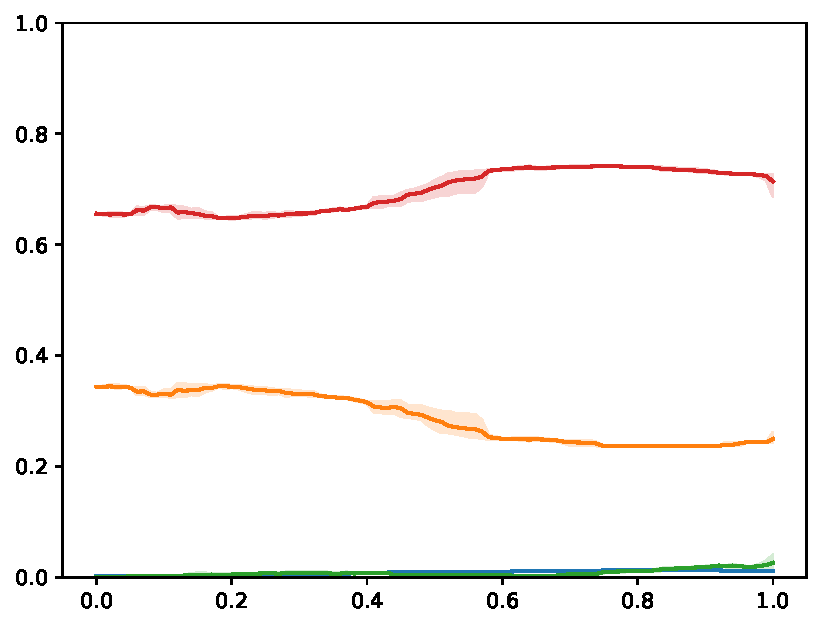
\includegraphics[width=.25\linewidth]{code/img/operation_count_zss_AT1-2.pdf} & 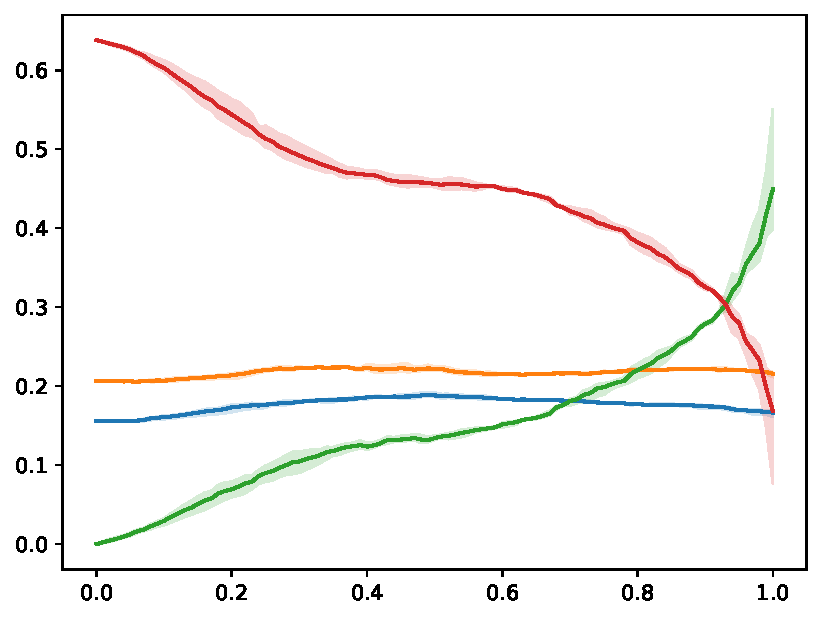
\includegraphics[width=.25\linewidth]{code/img/operation_count_zss_AT2.pdf} \\
    RRD      & 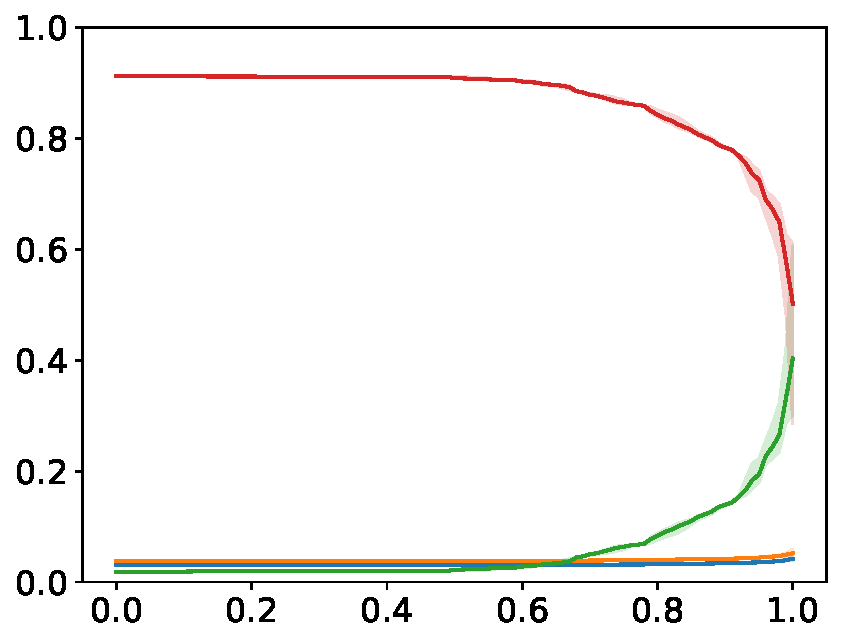
\includegraphics[width=.25\linewidth]{code/img/operation_count_rrd_AT1.pdf} & 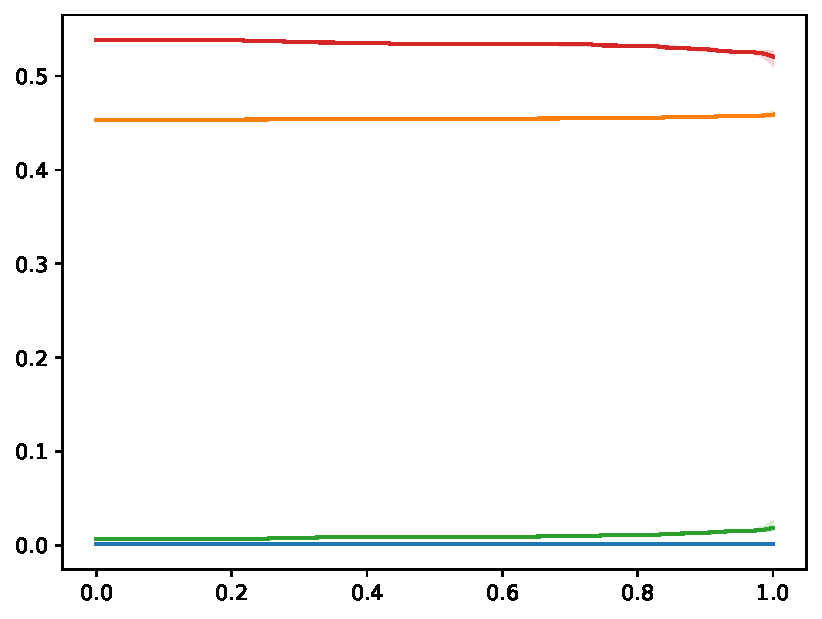
\includegraphics[width=.25\linewidth]{code/img/operation_count_rrd_AT1-2.pdf} & 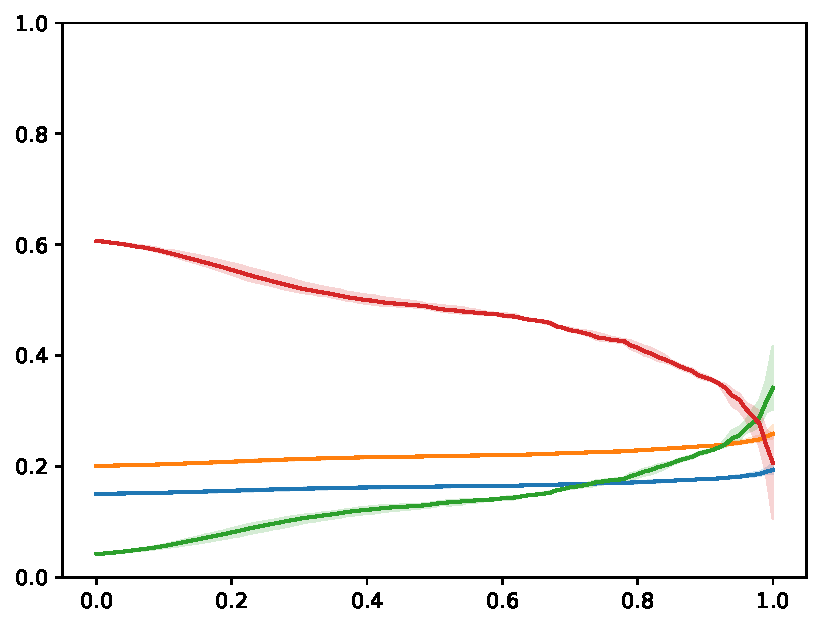
\includegraphics[width=.25\linewidth]{code/img/operation_count_rrd_AT2.pdf} \\
    MSD      & 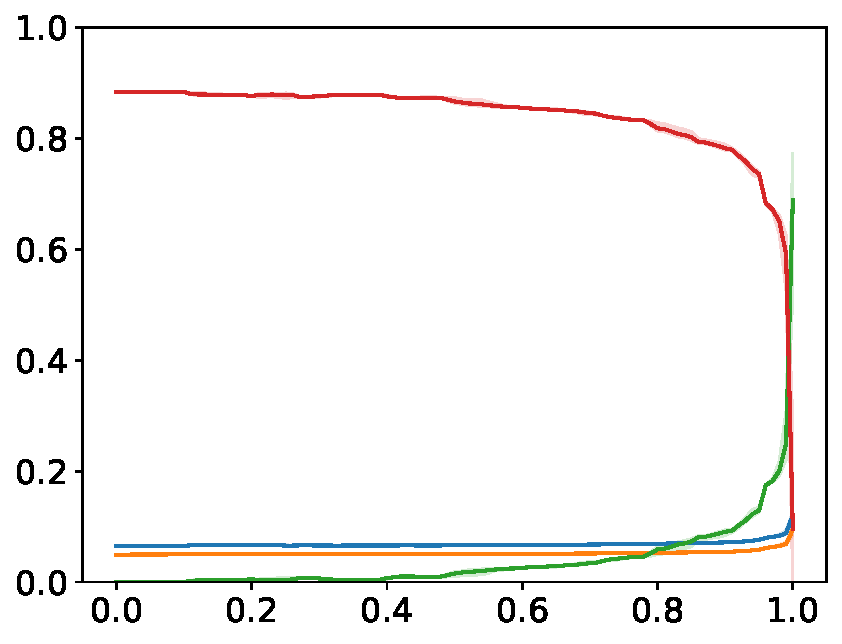
\includegraphics[width=.25\linewidth]{code/img/operation_count_ms_AT1.pdf}  & 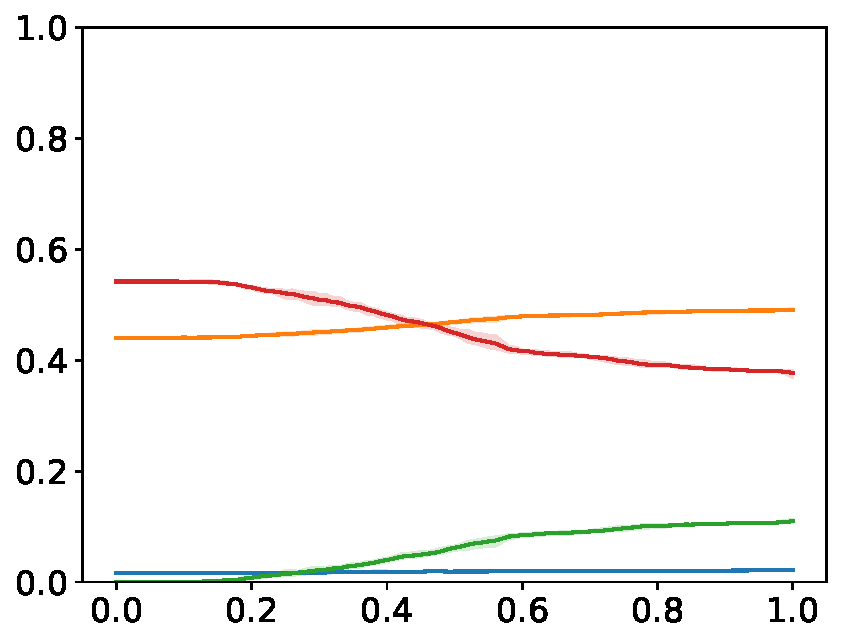
\includegraphics[width=.25\linewidth]{code/img/operation_count_ms_AT1-2.pdf}  & 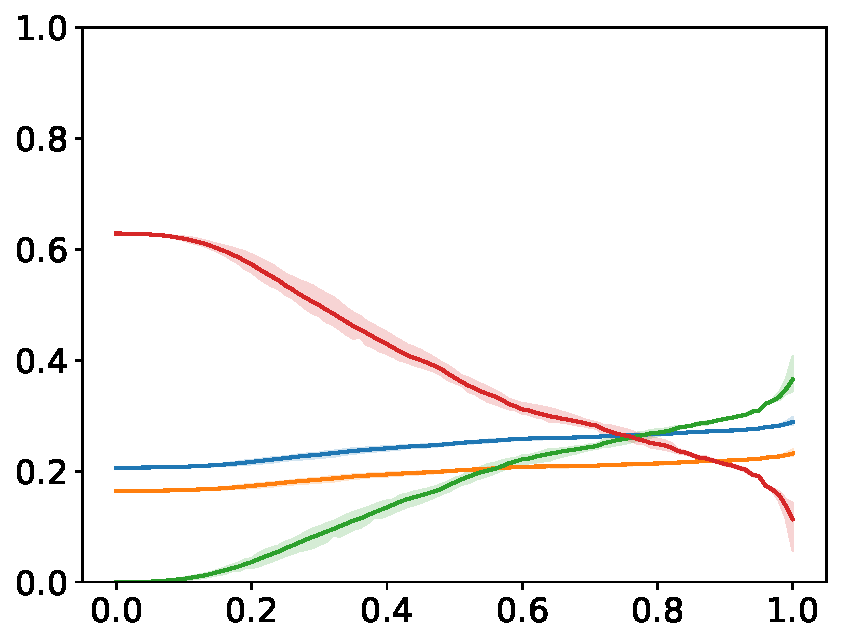
\includegraphics[width=.25\linewidth]{code/img/operation_count_ms_AT2.pdf}
\end{tabular}
\caption{Plots showing each type of modification operation as a percentage of the total number of operations for increasing similarity limit $\epsilon$. {\color{color1} \textbf{Blue}} indicates a removal operation. {\color{color2} \textbf{Orange}} indicates an addition operation. {\color{color3} \textbf{Green}} indicates a changing operation, and {\color{color4} \textbf{Red}} indicates a matching operation. }
\label{fig:operations}
\end{figure}


\begin{table}
    \begin{tabular}{lrrrr}
        \toprule
        Counterexample       & Label Distance & Tree Edit Distance & Radical Distance & Multiset Distance \\
        \midrule
        Refinement Switch    & 0              & 1                  & 1                & 3                 \\
        Extra Intermediate   & 1              & 1                  & 1                & 0                 \\
        Missing Intermediate & 1              & 1                  & 4                & 0                 \\
        Extra Leaf           & 1              & 1                  & 1                & 1                 \\
        Missing Leaf         & 1              & 1                  & 1                & 1                 \\
        Order Reversed       & 0              & 7                  & 0                & 0                 \\
        Changed Root         & 1              & 1                  & 1                & 0                 \\
        Changed Intermediate & 1              & 1                  & 1                & 0                 \\
        Changed Leaf         & 1              & 1                  & 1                & 1                 \\
        \bottomrule
    \end{tabular}
    \caption{The distances provided by each of the distance measurements. Each of these changes should result in an intuitive distance of 1.}
    \label{tab:counterexamples}
\end{table}








% \subsection{Measuring $\gamma(\Delta)$}

% \NS{Operations plot}

% \subsection{Finding optimal $\epsilon$}

% In Figure~\ref{img:similaritylimits}, we can see the effect of rising semantic similarity limit ($\epsilon$) on the average distance between each of attack tree 1 ($n=38$). Additionally, we can see the normalized Levenshtein distance plotted against the same semantic similarity limits. Finally, we can see the traditional Zhang and Shasha edit distance (based on string equivalence), which is unaffected by a similarity limit.

% \begin{figure}
% 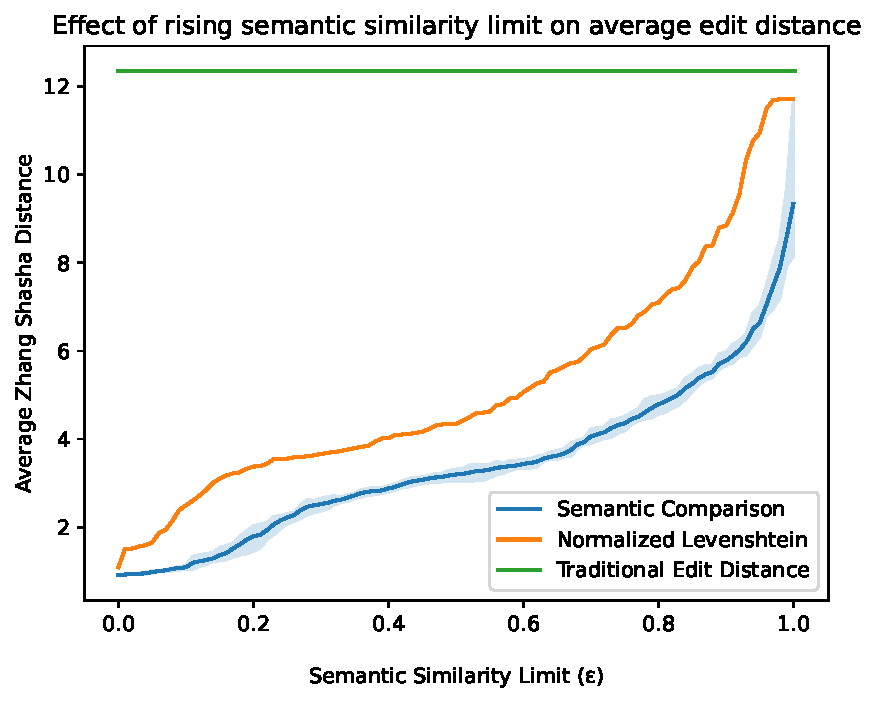
\includegraphics[width=\linewidth]{code/img/similaritylimits2.pdf}
% \caption{The average distance between the 38 experimental ATs per semantic similarity limit}
% \label{img:similaritylimits}
% \end{figure}

% \NS{Operations plot}


% \section{Effect of node flipping}

% \NS{plot showing average distance between 38 ATs with and without node flipping}


